\documentclass[
    12pt, % Schriftgröße
    ngerman, % für Umlaute, Silbentrennung etc.
    a4paper, % Papierformat
    oneside, % einseitiges Dokument
    headings=big, % Größe der Überschriften verkleinern
    listof=totoc, % Verzeichnisse im Inhaltsverzeichnis aufführen
    bibliography=totoc, % Literaturverzeichnis im Inhaltsverzeichnis aufführen
    index=totoc, % Index im Inhaltsverzeichnis aufführen
    captions=tableheading, % Beschriftung von Tabellen unterhalb ausgeben
    final % Status des Dokuments (final/draft)
]{scrartcl}
%anderes Layout mit {article} oder {scrartcl} erreichbar....

\usepackage[utf8]{inputenc} 
\usepackage[ngerman]{babel}                         %Landessprache Deutsch
\usepackage[T1]{fontenc}                            %Schriftformatierung
\usepackage[pdftex]{graphicx}                       %Implementierung von Grafiken
\usepackage{subfig} 
\usepackage[printonlyused,withpage]{acronym}        %Abkürzungsverzeichnis
%\usepackage{hyperref}                              %Erstellen von Hyperlinks
%\usepackage[figure]{hypcap}                        %Hyperlinks für Abbildungen

%Schriftdarstellung Darstellung optimieren
\usepackage{mathptmx} %Times New Roman
\usepackage{microtype}
\hyphenation{De-zi-mal-tren-nung} %Zeilenbrüche verwenden
\usepackage{color}
\usepackage{lmodern} % bessere Fonts
\usepackage{relsize} % Schriftgröße relativ festlegen
\usepackage{blindtext} %Packet Blindtext


\RedeclareSectionCommand[%
                         beforeskip = -24pt,% negativer Wert um den Einzug nach der Überschrift zu vermeiden
                        afterskip  = 8pt,% Abstand nach der Überschrift
                        indent  = 0pt% Einzug vor der Zahl der Überschrift
                         ]{section}
\addtokomafont{subsection}{\rmfamily\bfseries}
\RedeclareSectionCommand[%
                         beforeskip = -24pt,% negativer Wert um den Einzug nach der Überschrift zu vermeiden
                         afterskip  = 8pt,% Abstand nach der Überschrift
                         indent  = 0pt% Einzug vor der Zahl der Überschrift
                         ]{subsection}
\addtokomafont{subsubsection}{\rmfamily\bfseries}
\RedeclareSectionCommand[%
                         beforeskip = -24pt,% negativer Wert um den Einzug nach der Überschrift zu vermeiden
                         afterskip  = 8pt,% Abstand nach der Überschrift
                         indent  = 0pt% Einzug vor der Zahl der Überschrift
                         ]{subsubsection}
                         

% Seitenenlayout
\usepackage{geometry} %zunächst auf Standardeinstellungen belassen...
\usepackage{setspace} %für onehalfspacing später


%Schriftarten von Section, Chapter, Text etc. einstellen
\renewcommand{\rmdefault}{ptm}
\renewcommand{\sfdefault}{phv}
\renewcommand\familydefault{\rmdefault}
\addtokomafont{section}{\rmfamily\mdseries\Large \hspace*{-0.2cm}\vspace{-10pt}}
\addtokomafont{subsection}{\normalfont\large\rmfamily\bfseries\hspace*{-0.2cm}\vspace{-10pt}}

%Formatierung des Tabellen/Abkürzungsverzeichnis anpassen
%\usepackage{tocloft}
%\renewcommand{\cftfigpresnum}{Abbildung. }
%\renewcommand{\cfttabpresnum}{Tabelle. }

%\renewcommand{\cftfigaftersnum}{:}
%\renewcommand{\cfttabaftersnum}{:}

%\setlength{\cftfignumwidth}{2cm}
%\setlength{\cfttabnumwidth}{2cm}

%\setlength{\cftfigindent}{0cm}
%\setlength{\cfttabindent}{0cm}

%\renewcommand{\figurename}{Abb.}
%\renewcommand{\tablename}{Tab.}


%\renewcommand{\cftfigpresnum}{Abb. }
%\settowidth{\cftfignumwidth}{Abb. 10\quad}
%\setlength{\cftfignumwidth}{2cm}




% Kopf- und Fußzeile der ersten Seiten erstellen
\usepackage[automark]{scrlayer-scrpage}
\pagestyle{scrheadings}
\clearmainofpairofpagestyles{}
%\ihead{}
%\chead{}
%\chead{}{}
\ohead{\pagemark}






\begin{document}
\pagestyle{empty}
\begin{center}
\begin{tabular}{p{\textwidth}}
\begin{center}
\large {Private Fachhochschule für Wirtschaft und Technik \\
Bachelor of Engineering\\
Ausbildungsbetrieb: DIL Engineering GmbH}
\end{center}
\\
\begin{center}

\includegraphics[scale=1]{img/PHWT-Logo.jpg}
\end{center}
\\
\\
\begin{center}
\large{Praxistransferbericht zum Thema:}
\end{center}
\\
\begin{center}
\Large{Auslegung eines Druckbehälters nach Merkblatt AD2000}
\end{center}

\begin{center}
Beschreibung 1\\
Beschreibung 2
\end{center} \\
\begin{center}
vorgelegt von: 
\end{center}

\begin{center}
    \begin{tabular}{lll}
        \textbf{Steffen Specker:} & & Matrikelnr. 172897\\
        \end{tabular} 
\end{center}
\\
\\
\\
\begin{center}
\begin{tabular}{lll}
\textbf{Prüfer:} & & Herr Kray\\
\textbf{Abgabedatum:} & & 31.07.2022\\
\end{tabular}
\end{center}

\end{tabular}
\end{center}

%Verzeichnisse einrichten, römische Seitenzahlen in Kopfzeile

%\hypersetup{pageanchor=true} %Hyperlinks erstellen
%\setcounter{page}{1}
\pagenumbering{Roman}
\renewcommand{\thepage}{\Roman{page}}

%Absätze einstellen
\newgeometry{left=4cm, right=2cm, top=2cm}
\setlength{\parindent}{0cm}                     % Einrücken des Textes bei neuem Absatz
\setlength{\parskip}{0.5cm}                       % Vertikaler Abstand der Absätze (\par)
\doublespacing{}                               % Zeilenabstand

% Seitenränder für das Textdokument einstellen
\setlength{\headheight}{1.5cm}                    % Höhe Kopfzeile
\setlength{\voffset}{2.5cm}                     % Abstand Oberer Rand - Textfeld
\setlength{\topmargin}{-4.5cm}                  % Abstand Oberer Rand - Text oben
\setlength{\headsep}{0.5cm}                     % Abstand Kopfzeile - Text oben 
\setlength{\footskip}{2cm}                      % Abstand Fußzeile - Text unten
\setlength{\footheight}{1.5cm}                  % Höhe Fußzeile
%Abstand Gleitumgebungen zum Text
\setlength{\intextsep}{12pt}
\setlength{\textfloatsep}{12pt}


\tableofcontents
%\setcounter{secnumdepth}{3}
%\setcounter{tocdepth}{2}



\newpage
\listoftables % Tabellenverzeichnis
\vspace{2cm}
\listoffigures  %Abbildungsverzeichnis

\vspace{2cm}


\section*{Abkürzungsverzeichnis} 
\addcontentsline{toc}{section}{Abkürzungsverzeichnis} 

\begin{acronym}[Bash]
\acro{KDE}{K Desktop Environment}
\acro{dr}[Dr.]{Doktor}
\acroplural{dr}[Dres.]{Doktoren}
\acro{SQL}{Structured Query Language}
\acro{Bash}{Bourne-again shell}
\acro{JDK}{Java Development Kit}
\acro{VM}{Virtuelle Maschine}
\acro{I2C}[I²C]{Inter-Integrated Circuit}
\end{acronym}



\section*{Formelverzeichnis} 
\addcontentsline{toc}{section}{Formelverzeichnis} 
%\renewcommand{\listtablename}{}




 \cleardoublepage{}


%Ab hier beginnt das eigentliche Dokument
%Neue Kapitel mit \section

\newpage
\pagenumbering{arabic}
\ofoot{\thepage}
\ihead{}
\chead{}
\ohead{\thepage}



\section{Einführung in das Thema}

This will be an empty chapter
Vor Jahren waren \ac{KDE} die größten Vermittler der Welt. \\
Des lässt sich auch an xx feststellen. Der Mehrwert Bla Bla \blindtext\par


\blindtext{}

\subsection{Unterkapitel}
\blindtext{}
\subsection{Noch eins}
\subsection{Ein weiteres}

\newpage
\section{Grundlagen der Sterilisation und Rahmenbedingungen für die Konstruktion eines Dampfdruckbehälters}
\blindtext[1] \par
\blindtext[1.5] \par
\begin{figure}[htb]
    \centering  
    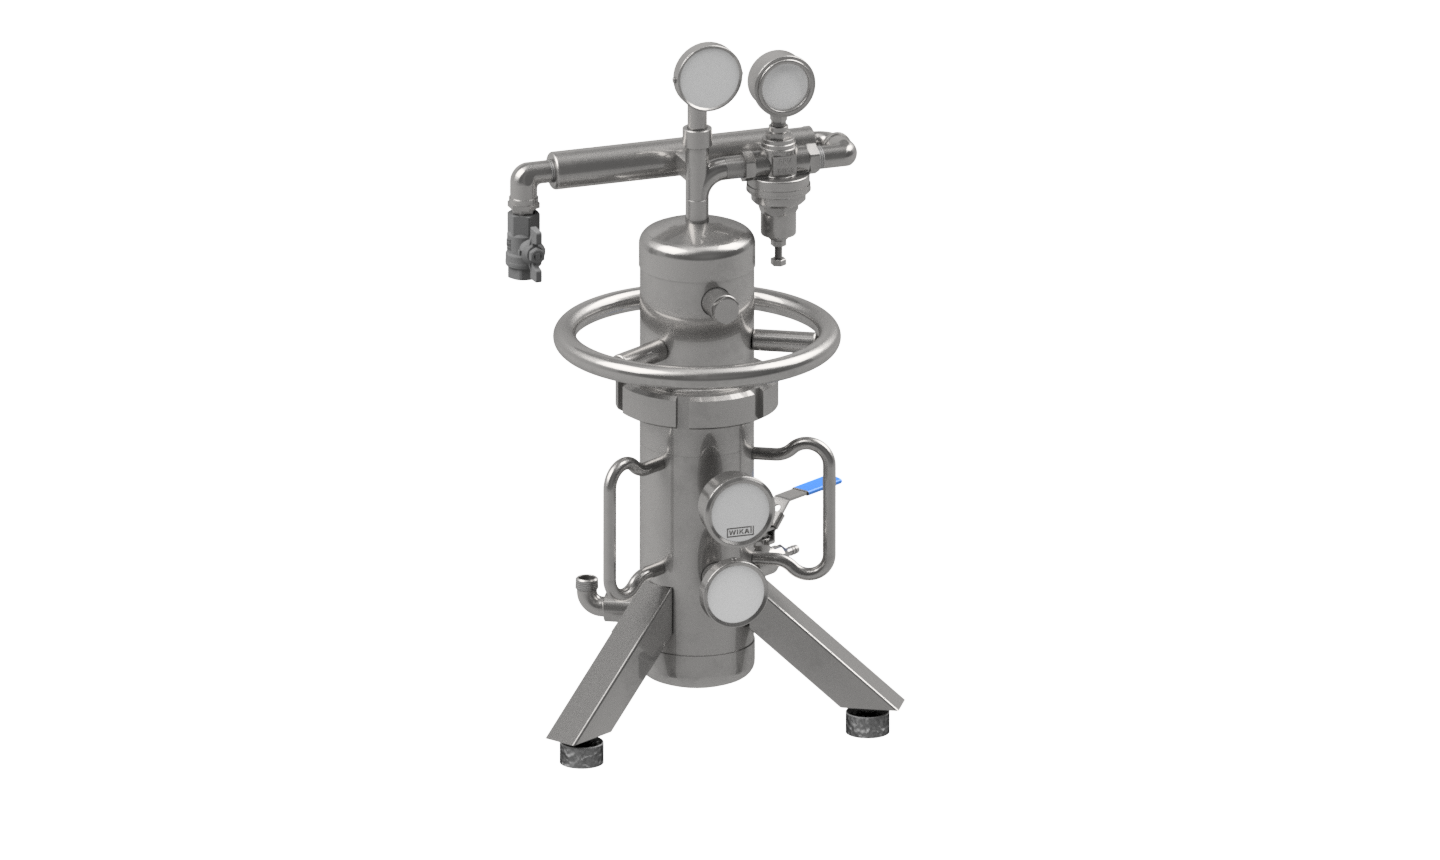
\includegraphics[keepaspectratio,width=\textwidth,height=\textheight]{img/render.png}
    \caption{3D Darstellung des Dampfdruckbehälters}\label{fig:render}
\end{figure}
\par
Dies ist auch in Abbildung \ref{fig:render} sehr gut zu erkennen (vgl. Abb.\ref{fig:render}).

\blindtext[1.2] \par

\end{document}

